% 保留 figures/balrogarch.png 的真实代码、游戏画面、接口与关系，仅覆盖说明标签。
\begingroup
\definecolor{chTenStrategyBg}{RGB}{162,218,173}
\begin{tikzpicture}
\node[anchor=south west,inner sep=0] (chTenArch) at (0,0) {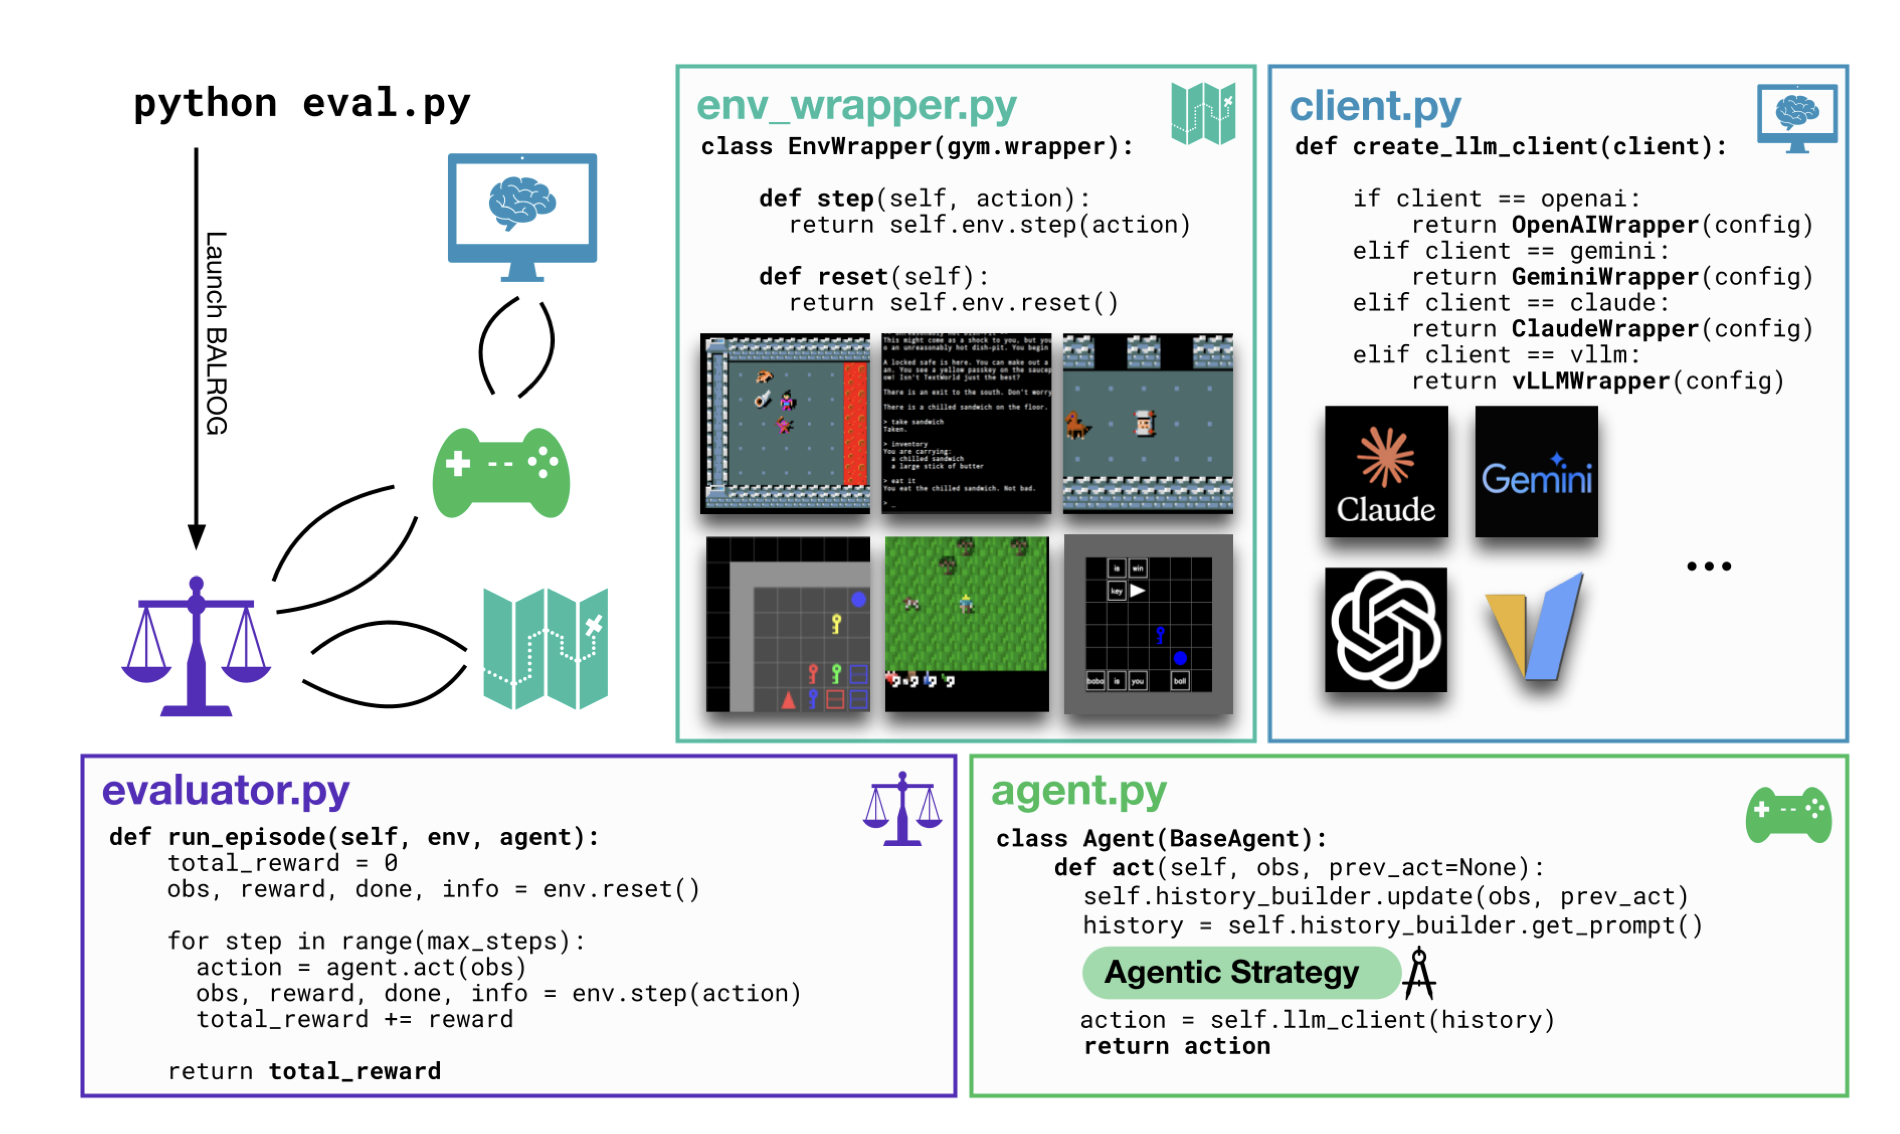
\includegraphics[width=\linewidth]{figures/balrogarch}};
\begin{scope}[x={(chTenArch.south east)},y={(chTenArch.north west)}]
\fill[white] (.107,.605) rectangle (.129,.802);
\node[rotate=-90,font=\small,inner sep=0] at (.115,.704) {启动 BALROG};
\fill[chTenStrategyBg] (.577,.128) rectangle (.724,.161);
\node[font=\bfseries\small,inner sep=0] at (.651,.144) {智能体策略};
\end{scope}
\end{tikzpicture}
\endgroup
